\documentclass[10pt,letterpaper]{article} % {{{
\usepackage[utf8]{inputenc}
\usepackage[english]{babel}
\usepackage{amsmath}
\usepackage{amsfonts}
\usepackage{amssymb}
\usepackage{graphicx}
\graphicspath{{tmp/}}
\usepackage{physics}
\usepackage{bbm}
\usepackage[dvipsnames]{xcolor}
\usepackage[margin=1in]{geometry}
\usepackage{booktabs}
\usepackage{float}

\newcommand{\eref}[1]{eq.~(\ref{#1})} 
\newcommand{\sref}[1]{sec.~\ref{#1}}
\newcommand{\fref}[1]{Fig.~\ref{#1}}
\newcommand{\tref}[1]{table~\ref{#1}}
\newcommand{\Eref}[1]{Eq.~(\ref{#1})} 
\newcommand{\Sref}[1]{Sec.~\ref{#1}}
\newcommand{\Fref}[1]{Fig.~\ref{#1}}  
\newcommand{\Tref}[1]{Table~\ref{#1}}

\usepackage{hyperref}
\hypersetup{
colorlinks=true,
linkcolor=blue,
filecolor=blue,      
citecolor=blue,
urlcolor=blue,
pdftitle={},
pdfauthor=author={Jose Alfredo de Leon},
}

\usepackage{tikz}

\usepackage[mathlines]{lineno}  \linenumbers \setlength\linenumbersep{5pt}
\usepackage[inline]{showlabels,rotating}
\renewcommand{\showlabelrefline}{\hrule width 0pt height 3ex depth 0pt}
\renewcommand{\showlabelfont}{\small\slshape\color{red!70}}
\usepackage[draft,inline,nomargin]{fixme} \fxsetup{theme=color}
\definecolor{jacolor}{RGB}{200,40,0} \FXRegisterAuthor{ja}{aja}{\color{jacolor}JA}
\FXRegisterAuthor{cp}{acp}{\color{blue}CP}
\FXRegisterAuthor{cd}{acd}{\color{purple}CD}

%\decimalpoint

\newcommand{\one}{\mathbbm{1}}

\newtheorem{theorem}{Teorema}
\newtheorem{proof}{Demostración}
\newtheorem{hypothesis}{Hipótesis}

\title{On ``The simplest 2D quantum walk detects chaoticity''}
\author{Jose Alfredo de Leon}
\date{\today}

\renewcommand{\labelenumii}{\arabic{enumi}.\arabic{enumii}}
\renewcommand{\labelenumiii}{\arabic{enumi}.\arabic{enumii}.\arabic{enumiii}}
\renewcommand{\labelenumiv}{\arabic{enumi}.\arabic{enumii}.\arabic{enumiii}.\arabic{enumiv}}

\newcommand{\rhoel}[2]{\rho_{#1,#2} \dyad{#1}{#2}}
\newcommand{\p}{p_{\text{error}}}


\begin{document}
\maketitle

\section{Summary}
In Ref.~\cite{alonso-lobo_2025_simplest}, Alonso-Lobo, Carlo, and Borondo 
investigate a two-dimensional discrete-time quantum walk (DTQW) inside a 
desymmetrized Bunimovich billiard (see Fig.~\ref{fig:bunimovich}) to identify 
signatures of chaos. 

The first indicator they examine is the level spacing distribution \( P(s) \) 
of the eigenphases of the DTQW step, expecting it to match the predictions of 
random matrix theory (RMT). However, the observed \( P(s) \) does 
not satisfactorily align with RMT predictions. Given that the system should 
exhibit chaotic behavior, I suspect there may be an issue related to the 
unfolding procedure or the presence of unaccounted symmetries. In fact, even 
for the rectangular billiard, the \( P(s) \) distribution does not conform to 
a Poisson distribution, which suggests that additional factors influencing the 
spectral statistics need to be considered.


\begin{figure}
\centering
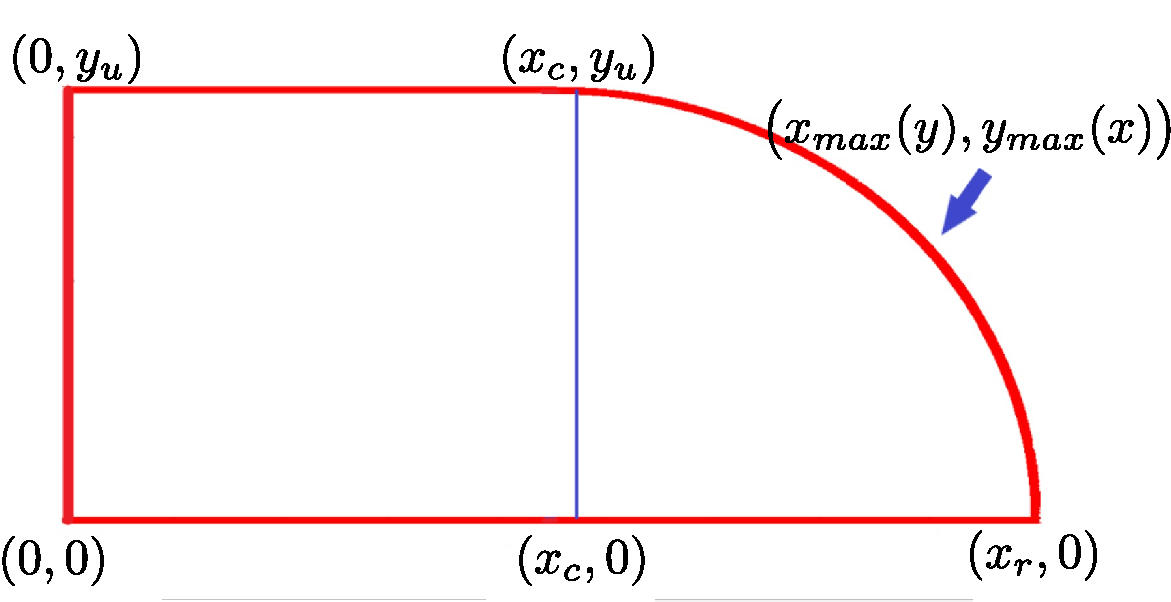
\includegraphics[width=0.7\textwidth]{bunimovich.pdf}
\caption{Desymmetrized Bunimovich stadium.
Figure taken and modified from~\cite{alonso-lobo_2025_simplest}.}
\label{fig:bunimovich}
\end{figure}

\section*{2D DTQW in a Bunimovich stadium}
One step of the DTQW in the desymmetrized Bunimovich stadium of 
Fig.~\ref{fig:bunimovich} in~\cite{alonso-lobo_2025_simplest} is given by:
\begin{equation}
    U = S_x C_2 S_y C_1,
\end{equation}
where \( S_x \) and \( S_y \) are the conditional shift operators that move the 
particle through the stadium, and \( C_1 \) and \( C_2 \) are the coin operators 
that introduce quantum superpositions in the internal degree of freedom. 

The shift operators conditionally displace the walker in the \( x \)- and \( y \)- 
directions, depending on the state of the internal coin degree of freedom:
\begin{align}
    S_x &= 
    \sum_{x=1}^{x_{\max}(y)-1} \dyad{x+1}{x}\otimes \one_y \otimes \dyad{0}_c +
    \sum_{x=1}^{x_{\max}(y)} \dyad{x-1}{x}\otimes \one_y  \otimes \dyad{1}_c + \\
    &\qquad  \dyad{x_{\max}(y)}\otimes \one_y \otimes \dyad{1}{0}_c + 
    \dyad{0}\otimes \one_y \otimes \dyad{0}{1}_c, \\
    %
    S_y &= 
    \sum_{y=1}^{y_{\max}(x)-1} \one_x \otimes \dyad{y+1}{y}\otimes \dyad{0}_c +
    \sum_{y=1}^{y_{\max}(x)} \one_x \otimes \dyad{y-1}{y}\otimes \dyad{1}_c + \\
    &\qquad 
    \one_x \otimes \dyad{y_{\max}(x)}\otimes \dyad{1}{0}_c + 
    \one_x \otimes \dyad{0}\otimes \dyad{0}{1}_c.
\end{align}
These operators ensure that the walker's movement is dictated by the coin state, 
which determines whether the displacement occurs forward or backward along each 
spatial direction.

The coin operators introduce quantum coherence by applying a unitary rotation in 
the internal spin space at each step:
\begin{equation}
    C_1 = \one_x \otimes \one_y \otimes 
    \mqty(\cos\alpha & \sin\alpha \\ -e^{i\pi/4}\sin\alpha & e^{i\pi/4}\cos\alpha),
    \quad 
    C_2 = \one_x \otimes \one_y \otimes 
    \mqty(\cos\beta & \sin\beta \\ -e^{i\pi/4}\sin\beta & e^{i\pi/4}\cos\beta).
\end{equation}
These unitary transformations mix the two internal states of the walker, playing 
a crucial role in generating interference effects that distinguish quantum walks 
from their classical counterparts.

This formulation defines a discrete-time quantum walk (DTQW) in which the quantum 
state of the walker evolves through a sequence of conditional shifts and internal 
coin rotations. The interplay between the shift and coin operations determines 
the statistical properties of the eigenphases of the evolution operator \( U \), 
which are key to analyzing the spectral signatures of chaos in the system.

\section{Distribution of Level Spacing Ratios $P(r)$}
Results from~\cite{alonso-lobo_2025_simplest} for the level spacing distribution 
$P(s)$ of the eigenphases of a DTQW step in the Bunimovich and rectangular 
billiards are shown in Fig.~\ref{fig:level:spacing:dist}. The authors argue that, 
although their statistics do not match the RMT prediction for the Bunimovich 
billiard nor the Poisson statistics for the rectangular billiard, the difference 
between both statistics distinguishes the chaotic and integrable cases.

\begin{figure}
\centering
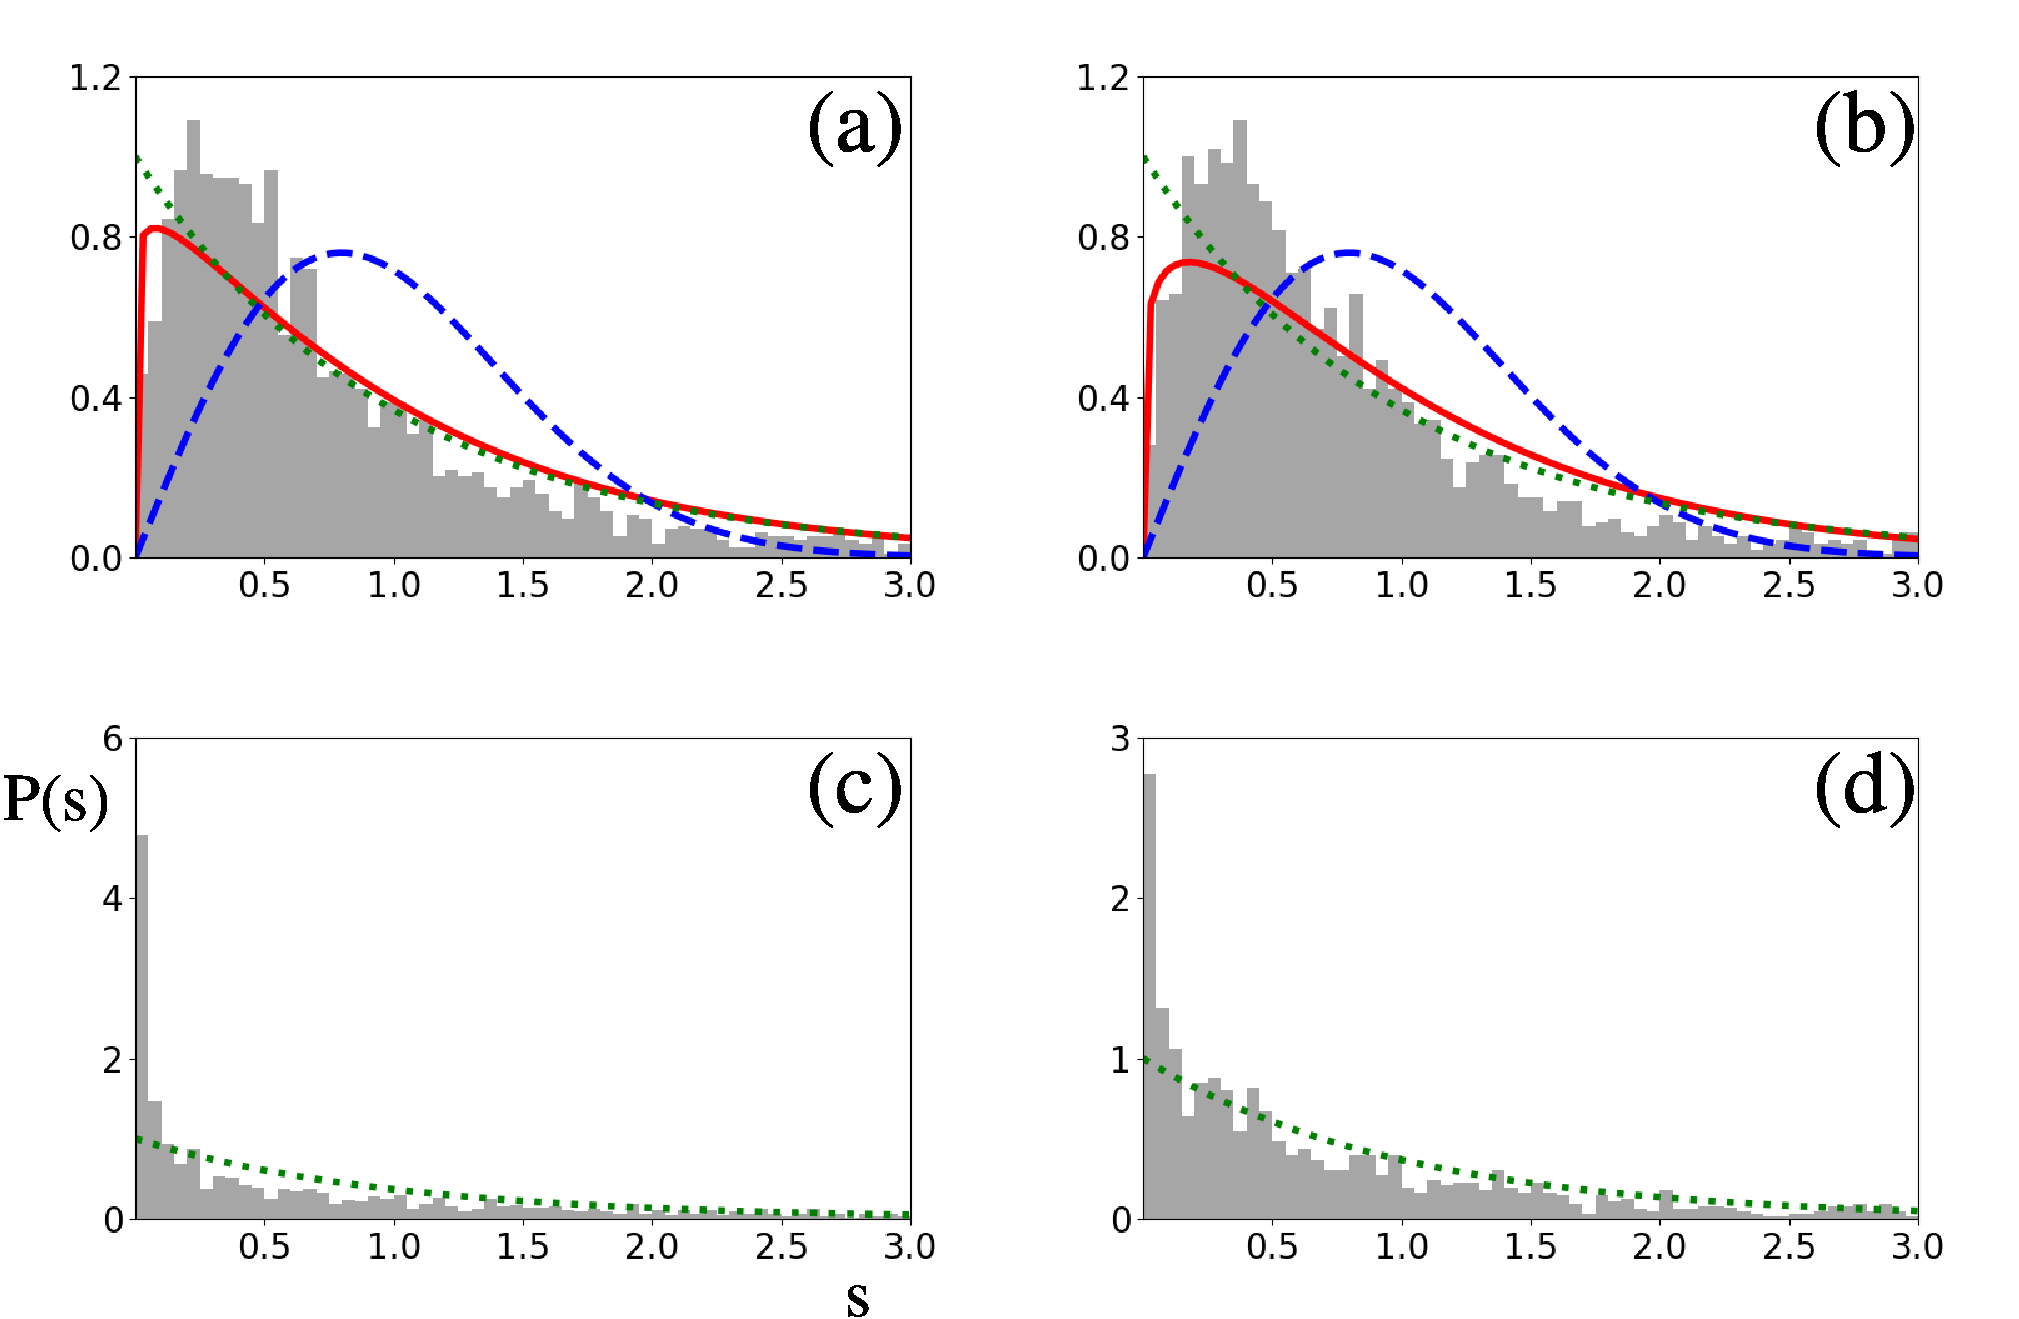
\includegraphics[width=\textwidth]{Figure4.png}
\caption{
Unfolded level spacing distributions $P(s)$. In (a) and (b) the Bunimovich stadium 
with coin angles $\alpha = \beta = \pi/4$, and $\alpha = \pi/4, \beta =\pi/3$, 
respectively. In (c) and (d) the rectangular stadium with coin angles 
$\alpha = \beta = \pi/4$, and $\alpha = \pi/4, \beta =\pi/3$, 
respectively. Green and blue dashed lines represent Poisson distribution and 
Wigner surmise for GOE ensemble, respectively, and red solid line is the best 
fit for the Brody distribution.
Figure taken from~\cite{alonso-lobo_2025_simplest}.}
\label{fig:level:spacing:dist}
\end{figure}

From my perspective, one should be able to match the RMT prediction for the 
Bunimovich billiard and Poisson statistics for the rectangular one. If not, there 
may be an issue with desymmetrization or the unfolding of eigenphases. Since no 
obvious symmetry exists in the case of different coins ($C_1 \ne C_2$), I initially 
suspected that the unfolding procedure was the problem. A way to circumvent this 
is to compute the level spacing ratio distribution $P(r)$, for which the RMT 
prediction has been derived analytically~\cite{atas_2013_distribution}. 

\begin{figure}
\centering
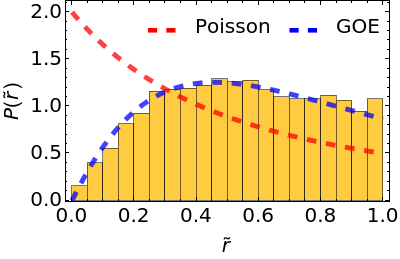
\includegraphics[width=0.7\textwidth]{Uv2_xc_50_alpha_Pi-4_beta_Pi-3.png}
\caption{Monedas de la v2 del arxiv~\cite{alonso-lobo_2025_simplest}. 
Dimensiones del estadio:
$|=\pi / 4$, $\beta=\pi / 3$. $x_c = 50$, $x_r=2 x_c$ y $y_u = x_c$.}
\label{fig:1}
\end{figure}

Figure~\ref{fig:1} shows the distribution $P(r)$ for $80\%$ of the eigenphases, 
taken from the middle of the spectrum. It closely matches the Wigner surmise for 
the GOE, clearly supporting the BGS conjecture. However, when computing the 
histogram of $P(r)$ for the case of equal coins $(C_1 = C_2)$, corresponding to 
Fig.~\ref{fig:level:spacing:dist}(a), a large number of occurrences of $\tilde{r} = 0$ 
were found, preventing the construction of a reliable histogram of $P(r)$. Since 
the unfolding should not be an issue in this case, I am inclined to think that an 
additional, unaccounted-for symmetry—besides the spatial one—is present. However, 
this symmetry is not obvious to me, and I have not yet been able to resolve the 
discrepancy with the Wigner surmise.

Notably, the left-most bin in Fig.~\ref{fig:level:spacing:dist}(a) and (c) is 
systematically taller than in Fig.~\ref{fig:level:spacing:dist}(b) and (d), further 
supporting the hypothesis of a missing symmetry when $C_1 = C_2$.  

\pagebreak
\section{Open questions}
\begin{itemize}
\item Is there a symmetry that prevents the spectral statistics from matching 
Poisson and RMT predictions?
\item Could it be a quasi-symmetry?  
\item If such a symmetry exists, how can it be identified?
\item The paper discusses other static signatures of chaos, such as the morphology 
of the eigenfunctions of a DTQW step. Would it be interesting to investigate 
dynamical signatures, such as the spectral form factor, survival probability, 
and Loschmidt echo?
\item While the original Bunimovich stadium problem is formulated as a 
single-particle system, in the DTQW formulation, one may consider the 
entanglement between position and spin degrees of freedom. Would it be 
worthwhile to investigate if it detects the integrable-chaos transition?
\end{itemize}

\bibliographystyle{unsrt}
\bibliography{referencias.bib}
\end{document}